% This is "sig-alternate.tex" V2.0 May 2012
% This file should be compiled with V2.5 of "sig-alternate.cls" May 2012
%
% This example file demonstrates the use of the 'sig-alternate.cls'
% V2.5 LaTeX2e document class file. It is for those submitting
% articles to ACM Conference Proceedings WHO DO NOT WISH TO
% STRICTLY ADHERE TO THE SIGS (PUBS-BOARD-ENDORSED) STYLE.
% The 'sig-alternate.cls' file will produce a similar-looking,
% albeit, 'tighter' paper resulting in, invariably, fewer pages.
%
% ----------------------------------------------------------------------------------------------------------------
% This .tex file (and associated .cls V2.5) produces:
%       1) The Permission Statement
%       2) The Conference (location) Info information
%       3) The Copyright Line with ACM data
%       4) NO page numbers
%
% as against the acm_proc_article-sp.cls file which
% DOES NOT produce 1) thru' 3) above.
%
% Using 'sig-alternate.cls' you have control, however, from within
% the source .tex file, over both the CopyrightYear
% (defaulted to 200X) and the ACM Copyright Data
% (defaulted to X-XXXXX-XX-X/XX/XX).
% e.g.
% \CopyrightYear{2007} will cause 2007 to appear in the copyright line.
% \crdata{0-12345-67-8/90/12} will cause 0-12345-67-8/90/12 to appear in the copyright line.
%
% ---------------------------------------------------------------------------------------------------------------
% This .tex source is an example which *does* use
% the .bib file (from which the .bbl file % is produced).
% REMEMBER HOWEVER: After having produced the .bbl file,
% and prior to final submission, you *NEED* to 'insert'
% your .bbl file into your source .tex file so as to provide
% ONE 'self-contained' source file.
%
% ================= IF YOU HAVE QUESTIONS =======================
% Questions regarding the SIGS styles, SIGS policies and
% procedures, Conferences etc. should be sent to
% Adrienne Griscti (griscti@acm.org)
%
% Technical questions _only_ to
% Gerald Murray (murray@hq.acm.org)
% ===============================================================
%
% For tracking purposes - this is V2.0 - May 2012

\documentclass{sig-alternate}

\begin{document}

\title{Continuous Experimentation to improve Value-oriented Software
\subtitle{[Extended Abstract]
\textit{Author's Guide to Preparing ACM SIG Proceedings Using
\LaTeX$2_\epsilon$\ and BibTeX} at
\texttt{www.acm.org/eaddress.htm}}}
%
% You need the command \numberofauthors to handle the 'placement
% and alignment' of the authors beneath the title.
%
% For aesthetic reasons, we recommend 'three authors at a time'
% i.e. three 'name/affiliation blocks' be placed beneath the title.
%
% NOTE: You are NOT restricted in how many 'rows' of
% "name/affiliations" may appear. We just ask that you restrict
% the number of 'columns' to three.
%
% Because of the available 'opening page real-estate'
% we ask you to refrain from putting more than six authors
% (two rows with three columns) beneath the article title.
% More than six makes the first-page appear very cluttered indeed.
%
% Use the \alignauthor commands to handle the names
% and affiliations for an 'aesthetic maximum' of six authors.
% Add names, affiliations, addresses for
% the seventh etc. author(s) as the argument for the
% \additionalauthors command.
% These 'additional authors' will be output/set for you
% without further effort on your part as the last section in
% the body of your article BEFORE References or any Appendices.

\numberofauthors{2} %  in this sample file, there are a *total*
% of EIGHT authors. SIX appear on the 'first-page' (for formatting
% reasons) and the remaining two appear in the \additionalauthors section.
%
\author{
% You can go ahead and credit any number of authors here,
% e.g. one 'row of three' or two rows (consisting of one row of three
% and a second row of one, two or three).
%
% The command \alignauthor (no curly braces needed) should
% precede each author name, affiliation/snail-mail address and
% e-mail address. Additionally, tag each line of
% affiliation/address with \affaddr, and tag the
% e-mail address with \email.
%
% 1st. author
\alignauthor
E.S. R{\o}mer\\
       \affaddr{University of Southern Denmark}\\
       \affaddr{5000, Odense}\\
       \affaddr{Denmark}\\
       \email{emroe12@student.sdu.dk}
% 2nd. author
\alignauthor
Nikolaj Schaldemose Reibke\\
       \affaddr{University of Southern Denmark}\\
       \affaddr{5000, Odense}\\
       \affaddr{Denmark}\\
       \email{nirei12@student.sdu.dk}
}
% Just remember to make sure that the TOTAL number of authors
% is the number that will appear on the first page PLUS the
% number that will appear in the \additionalauthors section.

\maketitle
\begin{abstract}
Contains abstract
\end{abstract}

% A category with the (minimum) three required fields
\category{H.4}{Information Systems Applications}{Miscellaneous}
%A category including the fourth, optional field follows...
\category{D.2.8}{Software Engineering}{Metrics}[complexity measures, performance measures]

\terms{
  Continuouse Experimentation,
  Value-oriented Software Development, 
  Value-based Software Development,
  Lean Software Development,
  Continous Delivery
}

\keywords{
  Continuouse Experimentation, 
  Value-oriented Software Development, 
  Value-based Software Development,
  Lean Software Development,
  Continous Delivery,
  Software Development,
  Project Management
}

\section{Introduction}
Doing business as a software company now, and expectedly increasingly in the future, needs to deal with increasing rapid changes in technology and competition. For a company to endure these changes in the business environment finding new strategies to distinguish themselves from their competitors is essential.\cite{stefan:valuebased}       
In order to accommodate these different company strategies and improve productivity a number of different software development processes have been developed. 
Throughout the last 60 years of software development, 5 different development processes categories have been created to accommodate the different business strategies and thereby improving the efficiency of the company. These categories can be seen below, arranged with oldest first.

\begin{enumerate}
\item \textit{Traditional Development.} Development processes like the waterfall model.
\item \textit{Agile Development.} Spans over development models like UP, RUP, Scrum, the V-Model and the spiral model.
\item \textit{Continues Development.} Development processes like Continuous Delivery and Continuous Deployment, which focusses on fast and short development cycles and quick a delivery.
\item \textit{Lean Software Development.} Development Processs which has become popular as speed has become more imporant. Additionally it focusses on manimizing loss in Software Development.
\item \textit{Continues Experimentation in value-oriented Software Development.} Development processes focussing on creating a minimal viable product through rapid development/delivery processes much like Continuous development.
\end{enumerate}

The general trend from the first to the last category is that the development process become more and more agile and iterative. This general trend can be view as attempts to overcome a number of general uncertainties or risk in software development.

As an example, take the jump from the traditional Waterfall to a agile framework like Scrum where the main purpose is to overcome these risks by using a more iterative and incremental approach\cite{sutherland:scrum}.

\begin{itemize}
\item \textit{Changes in requirements.} Changes in requirement are \textit{originally} thought of as risk of having "rework" costs, thereby posing the thread of exceeding the budget and potentially making the project a failure. As seen from Figure \ref{fig:vbseActivities} -\textit{Value-based adoption to change}, describing the activities of Value-Oriented Software Development, is there a paradigm shift in the view of these changes.
\item \textit{Risk of having the wrong requirements.} The risk of the identified set of requirements are wrong. Which can either lead to the developed system not for filling its purpose or the risk of changing requirements.
\item \textit{Risk of missing requirements.} If the identified set of requirement are lacking other essential requirements. This, depending on how late the missing requirements a discovered, can cause the major changes in the system and thereby introduce big costs to the project, or if the missing requirement are never discovered cause the system to be of on or little use.
\item \textit{Risk of not being the first.} The risk of the system release being too late. This can happen either by a competitor developing something faster or the organization/user solving the problem by other means.
\end{itemize}

On the last state of development is the value-oriented software development and its use of Continuous Experimentation to improve quality management. 

\subsection{Value-Oriented Software Development}
Value-oriented or Value-based Software Development (VBSE) focuses on reducing the waste of resources on activities with negative return investments. For instance, Boehm (2006) argues that the wasted effort by extensive testing could be as high as \$300 billion per year\cite{stefan:valuebased}.

VBSE originates from the "4+1" theorem represented on Figure \ref{fig:fouronetheorem}. This theorem states that a given company's enterprise will only be successful if it makes the success-critical stakeholders into winners. Therefore, the first step towards VBSE, is to identify \textit{all} stakeholders and  focus on those who are critical to the success.

The success-critical stakeholder (SCS) Win-Win theory at the centrer of the figure is used to decide which values are important and describes how to assure their success and realisation. The output of the additional four theories is the input for this decision making. Put simply, identify the values and determine their importance for the SCS. Further analyse how the identified SCS' values affect the decision making. Find and evaluate the dependencies and their impact on the values. Plan to adapt to changes and thereby control the realization of the value.\cite{stefan:valuebased}

\begin{figure}
\caption{The "4+1" theorem, by Boehm}
\centering
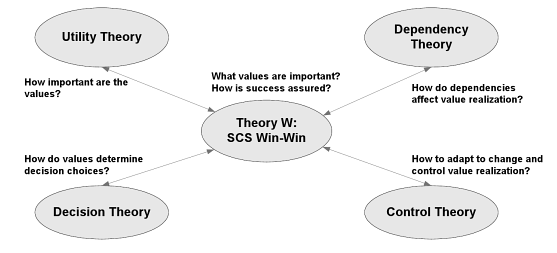
\includegraphics[scale=0.6]{Umlet/4+1theorem}
\label{fig:fouronetheorem}
\end{figure} 

The essence of VBSE and were it distinguish itself from the previous processes and strategies is that it does not operate with the same values-neutral approach. Where previous strategies treated every requirement, use case or defect with equal importance the VBSE seek to find a mutually satisfactory set of objectives for SCS' and company, and work these into a system. In other words, the value created from different requirements, use case, quality factors ect. are not of equal in size or importance. The size and importance of a value is defined by the success-critical stakeholders. Further, a item representing something valuable is not to be implemented if it is not important for the success of the enterprise. Derived from the W theory\footnote{The Win-Win theory of the "4+1" theory}, a successful enterprise is where the SCS becomes winners. 

This way of thinking manifests itself in a number of activities, which tries to maximize the value created on different levels of the engineering practices. These activities are:

\begin{itemize}
\item \textit{Value-based Requirement Engineering.} The process of eliciting the success-critical stakeholders for their value proposition with respect to the system. The goal here is to get a mutually satisfactory set of objectives for the system.
\item \textit{Value-based Architecting.} Designing a achievable architectural solution that captures the objectives for the system. 
\item \textit{Value-based Design and Deployment.} Establishing the techniques which ensures achieving system objectives with respect for the value considerations identified in the requirement engineering.
\item \textit{Value-based Verification and Validation.} The activity of ensuring that the system objectives are meet. Note that verification and validation is not interested in the requirements, but merely in whether the system creates the value proposed by the success-critical stakeholders.  
\item \textit{Value-based Planing and Controlling.} In general like traditional planning and controlling of cost and scheduling of the system, but extended to include the value delivered to the success-critical stakeholders.
\item \textit{Value-based Risk Management.} The activity of identifying risks to the project in order to prioritise, plan and control.
\item \textit{Value-based People Management.} In Value-Based Software Engineering, people management is crucial, to correctly identify objectives for the system, but also in order to ensure that expectations to the system does not exceed the actual objectives and goal of the system. 
\item \textit{Value-based adoption to changes.} Most Software engineering strategies view changes in  project requirements or quality factors as "rework costs" or quality costs which should be minimized. Value-based Engineering views these as changes in the environment of technology, markets, organizations and stakeholders. In a world contentiously and rapidly changing, the organization or stakeholder which is best at adopting to changes is the most successful. Since software is the premier technology to changes \cite{boehm:valuebased} Value-based engineering views it as opportunities for competitive success.
\item \textit{Value-based Quality Management.} Prioritising the desired quality factors in respect of the success-critical stakeholders.
\end{itemize} 

\paragraph{Quality management in VBSE}
Quality management in VBSE is focussing on prioritizing desired quality factors with respect to the stakeholders' value propositions. A crucial part of the quality management in VBSE is to identify what these factors are. Since software quality is multidimensional, it follows that the quality of a system can acceptable in one situation is not in odder. For instance a making a system with high efficiency but unknown or low reliability might be sufficient for a smart phone game application but as a system for a security system for a space program it is a no go. Further since quality costs money, narrowing down the which qualities really are important for stakeholders is a way to reduce wasted effort and money. In VBSE the quality management is concerned with identifying the most important qualities which should characterize the system and making sure that these are achieved to the extend where it meets the requirements of the stakeholders and no more. 
The main problem in VBSE is how to find out which quality factors are important, to which extend they should be meet. 

Further it is a problem in VBSE to verify that the quality goal identified is actually the correct once. Having a cap between the identified desired quality need and the \textit{true} quality need can lead to a business failure. 
Traditional development proposes to make studies of the user and the environment of the system to give evidence for a verification or rejection of a set of quality goal. But these studies can be costly and misleading, since the user does not always know what they want. Nor does a assessment of the environment prof whether one solution is better than another. Without any hard evidence, quality management in VBSE and other strategies can be a nasty business. Continuous Experimentation can be applied in this situation to reduce this risk of having wrong quality requirement. 
Continuous Experimentation is a strategy which is build on top of Continuous deployment.  

\subsection{Continuous Delivery and Deployment}
Continuous Delivery and Continuous Deployment are somewhat similar.
Continuous Delivery is a software engineering process focussing on a getting shorter development cycles, faster delivery and feedback, see Figure \ref{fig:deliverydeploment}. This is achieved by automating test and integration in a testing environment. Thereby making only the development and acceptance test manual. In continuous deployment the hole process after development is automated until the deployment in the production environment. There might still be manual work to do in the different tasks, like writing additional test, but the process of between the steps are completely automated.  

\begin{figure}
\caption{Continuous Delivery and Continuous Deployment in short}
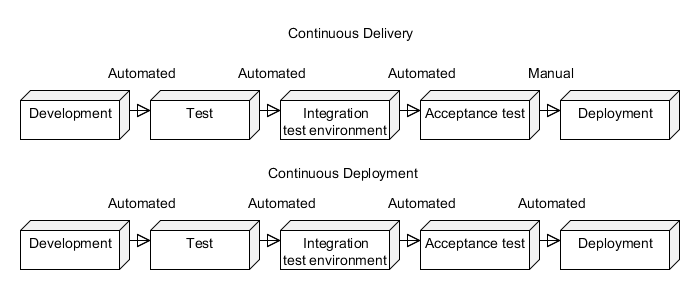
\includegraphics[scale=0.37]{Umlet/DeliveryandDeployment}
\label{fig:deliverydeploment}
\end{figure}


\subsection{Lean Software Development}
\label{lean}
Lean Software Developnment\cite{poppendieck:lean} was developed back in ?? and is based upon the following principles

\begin{enumerate}
\item \textit{Eliminate Waste.}
\item \textit{Amplify learning.} 
\item \textit{Decide as late as possible.}
\item \textit{Deliver as fast as possible.}
\item \textit{Empower the team.}
\item \textit{Build quality in.} 
\item \textit{See the whole.} 
\end{enumerate}

The following is a short description of the points found in the book \cite{poppendieck:lean}

\paragraph{Eliminate Waste}
Like Value-Oriented Software Development, Lean does not operate value-neutral. In Lean everything not adding value for the customer is considered wast to be minimized.
Waste is anything which does not directly add value upon the product. 

This is Design diagrams, which is not utilized by the developer or the project manager in any way. 
It is unused requirements, unused features or features which is not needed right now. 

Eliminating Waste is generally avoided by looking at each task done in a timeline for a project
and find any tasks or part of tasks which doesn't bring any value to the product and can be 
skipped for further processes or projects.
 
\paragraph{Amplify Learning}
Amplify Learning is generally described as using the Test Driven Development(TDD) approach in order to 
get instant feedback on success.
This means small iterations along with integration testing to quickly test if new features broke anything.
Though short development cycles, integration tests, re factoring sessions and quick user feedback, Lean development tries to maximize the learning of the project team members. This is done with the assumption that more knowledgeable and competent developers gives a better and faster end product.

\paragraph{Decide as Late as Possible}
For creative and design based tasks like software development a lot uncertainties are involved. 
The best approach for efficiency with big uncertainties is to make late decisions in order to have multiple
options, as not all options are good and there might be better options around. Further, does late decisions give a possibility of having more facts available to base the decision to be made on. 

The down side to this is, that the later a risk, uncertainty or problem is handled the bigger the change it enforces on the build system. Further, the higher the dependencies and entanglement between different components the greater is the risk of having to make major changes do to a late decision. This means that complex systems should support that parts of those systems can change in the late process
 of the development without the hassle to implement them.

\paragraph{Deliver as fast as possible}
Deliver as fast as possible is partly connected to the Eliminate Waste. 
Back in time it was more valuable to delay software and increase the quality, along with carefully making 
the right decisions.

Today it it more valuable to move fast and the cost of software has changed to the cost of human hours. 
These changes in the field has made it more important to elimate waste and deliver as fast as possible 
by just fulfilling the required terms.
As mentioned in \textit{Amplify learning} does Lean have short  development cycles which lowers the time until feedback can be gathered. Through fast feedback Lean Development tries to lower the four general risks seen in Figure \ref{fig:generalrisks}.

\paragraph{Empower the team}
Empower the Team, is for Lean Software Development the process of enlightning the entire team of the 
details of the project and thereby increase the quality by having every developer on the same side. 

These empowerings are archived by having the individual developers talk together in meetings telling
about what they have to do, combined charts which shows how the software is improved.

\paragraph{Build integrity in}
To Build Integrity in, means that it should be possible to extend the software for future requirements 
as software generally has to adapt to the moving world and additonally be easy to maintain to reduce waste.
Lean encourage the developer to do Re-factoring both to amplify learning among the developers, but also to keep the code base clean of unused functionality. In addition, is one of the goals of the re-factoring process to ensure flexibility and lower dependencies in between components and modules.  


\paragraph{See the whole}
The principle `See the whole` covers how to avoid suboptimality of the software. 
It is described as developers tend to do the features at which, they are specialized into.
This leads to parts of the systems being really good and other parts to be suboptimal.
Lean attempts to reduce suboptimal in a product by standardizing different stages in the iterations and make sure that every team member knows what the focus of this exact stage is. In addition, in bigger project where multiple different teams are working on the same end product intercommunication is highly important. This intercommunications is for ensuring the flexibility and assembly of different components is sufficient. This manifests itself in the Lean saying "Think Big, act small, fail fast and learn rapidly" \cite{poppendieck:lean} 


\subsection{Continuous Experimentation}
The section Continuous Experimentation is mainly grounded in the paper \cite{bowman:reasoning}.
The development approach is mainly inspired from Lean Development which focus upon the utilization of the budget to earn the most profit.

The Overall concept of Continous Experimentation is to iteratively `Build, Measure Learn` which is
decomposed into the following processes: 
\begin{enumerate}
\item Assumption
\item Hypothesis
\item Design of Minimal Viable Product
\item Integration
\item Feedback
\item Analyse Data
\end{enumerate}

An easier view of the process can be found on fig. \ref{fig:continuousdev}

\subsubsection{Assumption}
\label{cx:assumption}
The Initial process for continuous experimentation is the Assumption.
In the Assumption phase an idea is created, which is a change or extension to the current software.

\begin{figure}
\centering
\caption{Continuous Experimentation in short}
\label{fig:continuousdev}
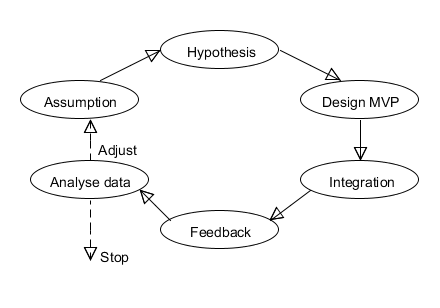
\includegraphics[scale=0.5]{Umlet/conexp}
\end{figure}

\subsubsection{Hypothesis}
\label{cx:hypothesis}
In the Hypothesis phase the focus is upon quality metrics which can be measured.
it it absolute crucial to the whole process that all these quality measures is measureable in order to figure 
out the value of the experiment, and find a direct statistical connection to it. 

In the Hypothesis the goal of the experiment is being described in measureable terms by these quality measures. 
The quality measures is not only software based, but also user experience is put into the hot seat in this 
phase, just as Lean Software Development\footnote{\label{see-lean}see section \ref{lean}} where waste is reduced, and value is maximized, the only real measureable value is in the end the user experience. 

If the user Experience qualities has totally failed, there is no value to the product and therefore there is 
no product.

\subsubsection{Design Minimal Viable Product}
\label{cx:design}
The Design of the Minimal Viable Product is usually done fast and tested following a `Test Driven Development`
approach, to ensure quality and non-breakability. 
This is a treat inheritated from Lean Software Development\footnotemark[\ref{see-lean}].

\subsubsection{Integration}
\label{cx:integration}
In order to use Continous Experimentation it is not sufficient to run only one version of software in 
production to be successful as it would take too long to test all the parallel experiments which has been
created and has entered the `Integration` phase. 

There is a number of ways to get around this issue of multiple versions. 
Either the server can decide which version is offered or the client can decide.

A version should be offered to a subset of the users, meaning not all users will be exposed to the 
new feature, but enough to show how it affects the software product.

Using only a subset of the users for an experiment also means that multiple experiments can be tested in 
parallel to different subsets. For some experiements the subsets might be able to handle a intersection of 
the subsets. 

\subsubsection{Feedback}
\label{cx:feedback}
In order to measure anything from the experiments it is crucial to collection user data.
The whole framework of the software system has to support collection of user data, both in order to see how 
the software system is doing in general, but also how experiments differences from the current master version.

The collection of data can be very different depending on the case and the product. 
For a webshop an experiment for a visual new feature could be tracked by collecting data about the amount 
of transactions made, what the transactions included and a clipmap of there the users clicked on the page.

These information would in contrast to the master version, be easily to distinguish from the statistics if 
the experiment caused any change.

\subsubsection{Data Analysis}
\label{cx:analyse}
Once data has been collected over a period of time. The collected data will be used to either accept or reject
the hypothesis. 
If the data collected has shown that all the quality measures has been met for the experiemnet, 
the experiment will be added to the master version as it has added value to the product.

On the other hand, if the data collected shows that the experiement has failed to fulfill the hypothesis 
the assumption will be re-evaluated for one of two things as seen in fig. \ref{fig:validation}. 
\begin{enumerate}
\item The Experiment will be archived and will not be used
\item The Experiment will have changed it hypothesis and can then be re-examined in order to fulfill the new 
hypothesis or not which may make it a candidate for the master version in the next iteration.
\end{enumerate}

\begin{figure}
\centering
\caption{Workflow of validation in Continuous Development}
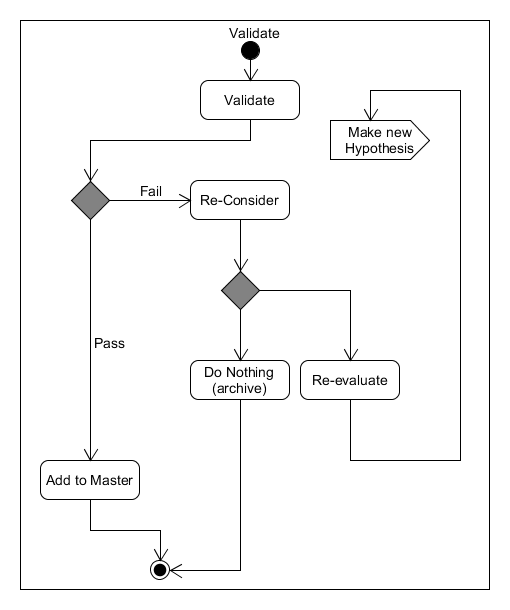
\includegraphics[scale=0.4]{Umlet/ValidateActivity}
\label{fig:validation}
\end{figure}

\section{Discussion}
In the previous sections, this paper have been looking into a number of different development processes in order to gain the information needed to understand what Continuous Experimentation is about. Further have the paper outlined the process of Continuous Experimentation. The Following sections will highlight some of the drawbacks of Value-oriented development and how Continuous Experimentation can be applied to counter these drawbacks. The first section \textit{Consequences of Value-oriented Software Development} will briefly discuss these drawbacks. 


\subsection{Consequences of Value-Oriented Software Development}
Value-Oriented Software Development non-neutral-value understanding of features, quality and system elements, gives project managers a new tool to maximize productiveness and ensure the success of a project. With the ideology of one system value not being equal to another, Value-Oriented Software Development gives the opportunity to focus on the development of what in the system will create the biggest value. Further, will it allow manager to prioritize the different features accordingly to how valuable they are. Lastly, by having a measure on how valuable a given value is the project manager can discard all features where there is no positive return of investment and guide his/hers decisions on what will maximize the value.  

As insinuated in \textit{Value-Oriented Software Development}, does Value-Oriented Software Development impose some risk to the project. 
Firstly, the method of Value-Oriented Software Development itself poses a risk, because it can be hard to quantitatively calculate and measure the values of different features, components or qualities. This can lead to decision being made on wrong numbers or decisions to be biased or partial. Besides taking a wrong turn based on faulty calculation there is a number of risks in Value-Oriented Development, these are:  
\begin{itemize}
\item \textit{The assumptions of the environment and current state wrong.} Having wrongly or incomplete perception of the environment can lead to making the wrong decision and or focus in the development.  
\item \textit{The gathered set of requirements/features is incomplete.} If the set requirement are incomplete the decision of what creates value in a product will be incomplete as well. Therefore it poses a risk for the project.
\item \textit{Wrongly identified success-critical stakeholders.} For the Win-Win theory to work, it is a pre requirement that all success-critical stakeholders are identified. If one or more success-critical stakeholder is missing it will introduce the risk of weighting the requirements wrongly. 
\end{itemize} 





\subsection{Synergy of CX and VoSD}
\subsection{Profit!}

\section{Conclusions}
%\end{document}  % This is where a 'short' article might terminate

%ACKNOWLEDGMENTS are optional
\section{Acknowledgments}

After all Coffee isn't that bad 

%
% The following two commands are all you need in the
% initial runs of your .tex file to
% produce the bibliography for the citations in your paper.
\bibliographystyle{abbrv}
\bibliography{sigproc}  % sigproc.bib is the name of the Bibliography in this case
% You must have a proper ".bib" file
%  and remember to run:
% latex bibtex latex latex
% to resolve all references
%
% ACM needs 'a single self-contained file'!
%
%APPENDICES are optional
%\balancecolumns


\end{document}
